\section{METHOD}\label{sec:method}
This section explains how supervisory control synthesis is used to perform the case studies described in \cref{sec:case_studies}.
First the existing architecture to control the robot is explained.
This control, already in place, is used as the basis on which the supervisory control, presented in this paper, is added.
The system architecture for this supervisory control implementation is discussed next.
The design choices made to achieve a working supervisor implementation on the robot, that provides the benefits laid out throughout the paper, are discussed as well.\\

As shown in \cref{fig:system_architecture}, the system architecture used in the case studies can be divided in two parts: existing robot control implementation and the supervisory control implementation.
Since this research focuses on the supervisory control of autonomous robots in general, the existing robot control implementation is only explained where it interacts with the supervisor.\\

The low-level control of the robot is written in \texttt{C++} and leveraged by a set of \texttt{robot\_skills} written in \texttt{Python}.
The \texttt{robot\_skills} \textit{"provide interfaces to all parts of a robot: its base, arms, head, perception, worldmodel, speech system, etc."}~\cite{amigo_github}.
The robot abstraction layer provided by \texttt{robot\_skills} is used by \texttt{robot\_states}, which in turn uses SMACH finite-state machines to describe skills regarding navigation, manipulation and so forth.
Finally, the skills in \texttt{robot\_states} are used in a SMACH-based task description, called a challenge.
% The case studies used in this research take the place of challenges.
An example of this interaction is shown in \cref{fig:robot_states_skills}, taken from the \texttt{tue\_robotics} repository.
The code in the \texttt{tue\_robotics} repository~\cite{amigo_github} contains further information about the system architecture of the existing robot control implementation.\\

\begin{figure*}
  \centering
  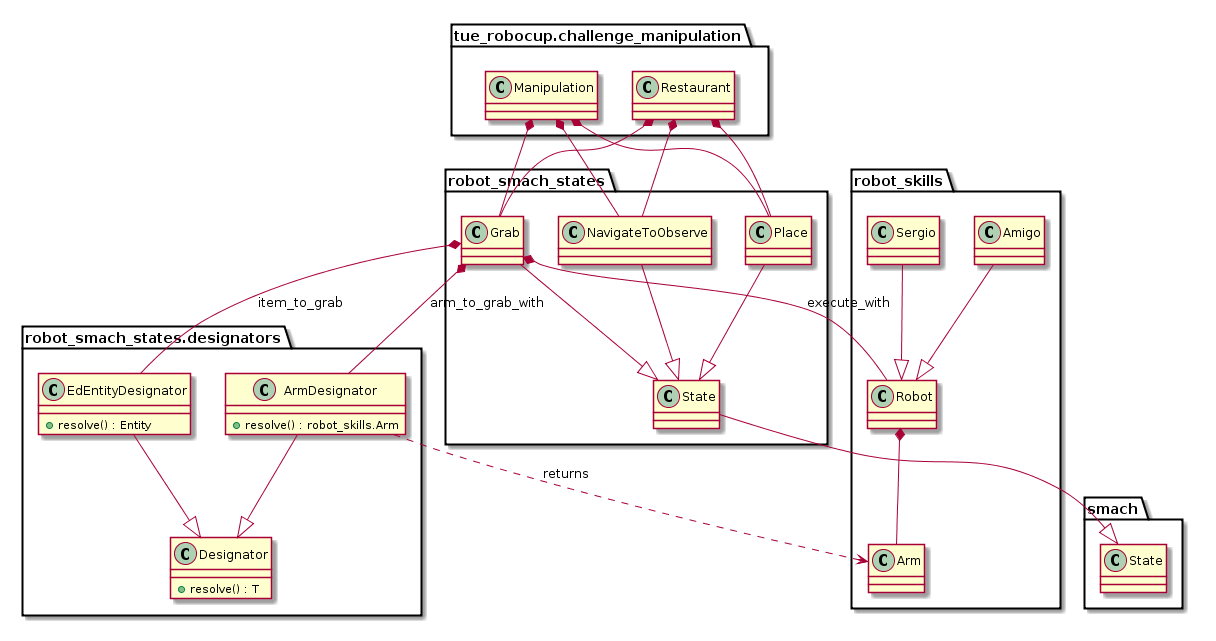
\includegraphics[width=0.9\textwidth]{robot_skill_states.png}
  \caption{Example interaction robot layers}\label{fig:robot_states_skills}
\end{figure*}

The model of the robot and requirements are created in CIF 3~\cite{cif3} and based on them a supervisor was synthesized. 
The CIF 3 language is designed to efficiently describe a plant, in this case Amigo, and its requirements, with automata or state-based expressions.
An example plant automaton is shown in \cref{code:armCIF} of Appendix~\ref{sec:code}. 
\todo[disable]{all models that are relevant or different, show skill task safety}
One recognizes the locations, including the initial and marked keywords, transitions represented by edges and declarations of (un-)controllable events as mentioned in \cref{sec:supervisory_control}.
This CIF automaton is shown graphically in \cref{fig:automaton_arm_l}.
An example of a requirement automaton in CIF and its graphical representation are shown in, respectively, \cref{code:safeArmCIF} of Appendix~\ref{sec:code} and \cref{fig:automaton_safe_arm_l}.
This safety requirement prevents collisions of the arms.
When a collision is detected on the path planned by the robot, the supervisor cancels the current plan and plans a new one.
A more detailed explanation of these models can be found in~\cite{jorrit_github}.
For this paper a set of models and requirements was created, that contained all the necessary components to execute the case studies, this can be expanded on in later research.\\

CIF uses the algorithm~\cite{CIF_algo} to synthesize a maximal permissive, controllable and non-blocking supervisor.
The output of the CIF synthesis procedure is a supervisor described in the CIF modelling language, but the CIF tool set provides conversions to other languages as well~\cite{cif3_c99}.
To integrate this supervisor with the robot and the existing control implementation, the supervisor was converted to \texttt{C} code, utilizing the tool from~\cite{cif3_c99}.
The CIF converted \texttt{C} code is available to the user as a library, which is used in this paper as follows:
the CIF generated supervisor library exposes two entry point functions to the user: \texttt{void EngineFirstStep()} and \texttt{void EngineTimeStep()}.
\texttt{void EngineFirstStep()} initializes all the data and executes the events that are not blocked by the supervisor, before the first time step.
\texttt{void EngineTimeStep(double delta)}, which needs to be called regularly by the user, updates time-dependent equations and variables in the model with time \texttt{delta} and then executes the events that are not blocked by the supervisor.
Guards for these events can depend on variables that can be set by the user, by calling a function with the name of the variable.
Looking at the example in \cref{fig:automaton_arm_l,fig:automaton_safe_arm_l}, the variables that can be set from the calling program are: \texttt{collision\_on\_path} (\(cp\)), \texttt{path\_valid} (\(pv\)) and \texttt{goal\_reached} (\(gr\)).
The function names would be, respectively, \texttt{void collision\_on\_path()}, \texttt{void path\_valid()} and \texttt{void goal\_reached()}.\\
The supervisor needs to interact with the robot, so the robot actually executes the actions imposed by the events of the supervisor.
To this end, the CIF generated supervisor library exposes a callback function \texttt{void InfoEvent(Event\_ event, BoolType pre)}.
This callback function needs to be defined in the program using the library and is called every time an event is about to, or has been executed.
In the case studies described in this paper, the function is defined in python and will execute the \texttt{robot\_states} or \texttt{robot\_skills} relevant to the event.
This function definition and other communication functions between the supervisor and the existing robot control are implemented in a file called the python wrapper.
It is important to note that to ensure that the supervisor knows if the robot is actually executing, or has completed, the task requested by the supervisor, variables need to be included so the robot can report back its current state.
CIF provides the \texttt{input} variable type, to facilitate this.
These are variables that the robot needs to assign to, after every time step, using the function \texttt{AssignInputVariables}\\
 
The complete code containing the CIF models, the supervisor and the python wrapper of the case studies, and a detailed plan on how to compile them, can be found in the code repository~\cite{jorrit_github} of the project described in this paper.
The repository also contains a detailed usage description of the CIF models, the supervisor, the python wrapper and the SMACH implementation, so the method can easily be integrated in further research.\\

Concerning the application scope of supervisory control in the case studies, the supervisor can be applied to different abstraction levels.
Applying supervisory control to the low-level control of the robot is difficult, because the control is mainly continuous and not discrete-event based.
The lowest level of abstraction supervisory control was applied to in this research was on the skill level, using the skill requirements. 
They control one component of the robot, but only the discrete events of that component.
This abstraction level was chosen, because the skills can still be described by finite-state machines and are discrete-event based.
One level of abstraction higher are the safety requirements. 
They can span multiple components and block events from one component based on information from another. 
The highest abstraction level supervisory control was applied to in this research was on the task level, using the task requirements.
They only control the order of skill events the robot executes and control nothing of the skills themselves.\\

\subsection{LIMITATIONS}
The presented case studies and method show the benefits that supervisory control synthesis can offer to autonomous robots.
There are, however, properties or benefits supervisory control synthesis can offer, that could not be translated to the dynamic environment of autonomous robots.\\

Non-blockingness, for example, can be used to ensure that a system is able to reach a certain state.
In robotics this could mean that a robot would never execute an action that would block a path, the robot later needs to navigate.
Another example where the non-blockingness property could prove useful, is a low-level implementation of supervisory control synthesis for control of the arms.
One can imagine it could be beneficial to make sure the arms never block each other when reaching for an object.
Both of these examples are impossible to implement with the method described in this paper, because of the dynamic environment the robot operates in.
This is caused by the fact that the supervisor is synthesised off-line and therefore cannot predict what happens when the robot enters an unknown environment.
There exist on-line supervisory control synthesis techniques~\cite{online_partially_observed,online_near_optimal,online_sup_rep_obs_sub}, that could prove useful in future research.\\

Another limitation is that CIF is a clear and concise language, but also somewhat limited.
Strings are not allowed as variables when performing supervisory control synthesis, for example, which is a big limitation when trying to describe a list of items to be picked up.\\